\newpage
\section{Fully assembled submodule}


The fully assembled submodule is shown in figure \ref{fig:real_submodule}.
\begin{figure}[H]
\includegraphics[width=1\linewidth]{submodule}
\caption{Designed and real assembled submodule.}
\label{fig:real_submodule}
\end{figure}


MEMS driver board (left) and SiPM board (right) are joint via flexible PCB (Fig. \ref{fig:flex_PCB}), the back of which has a connector for connection to the control board.

\begin{figure}[H]
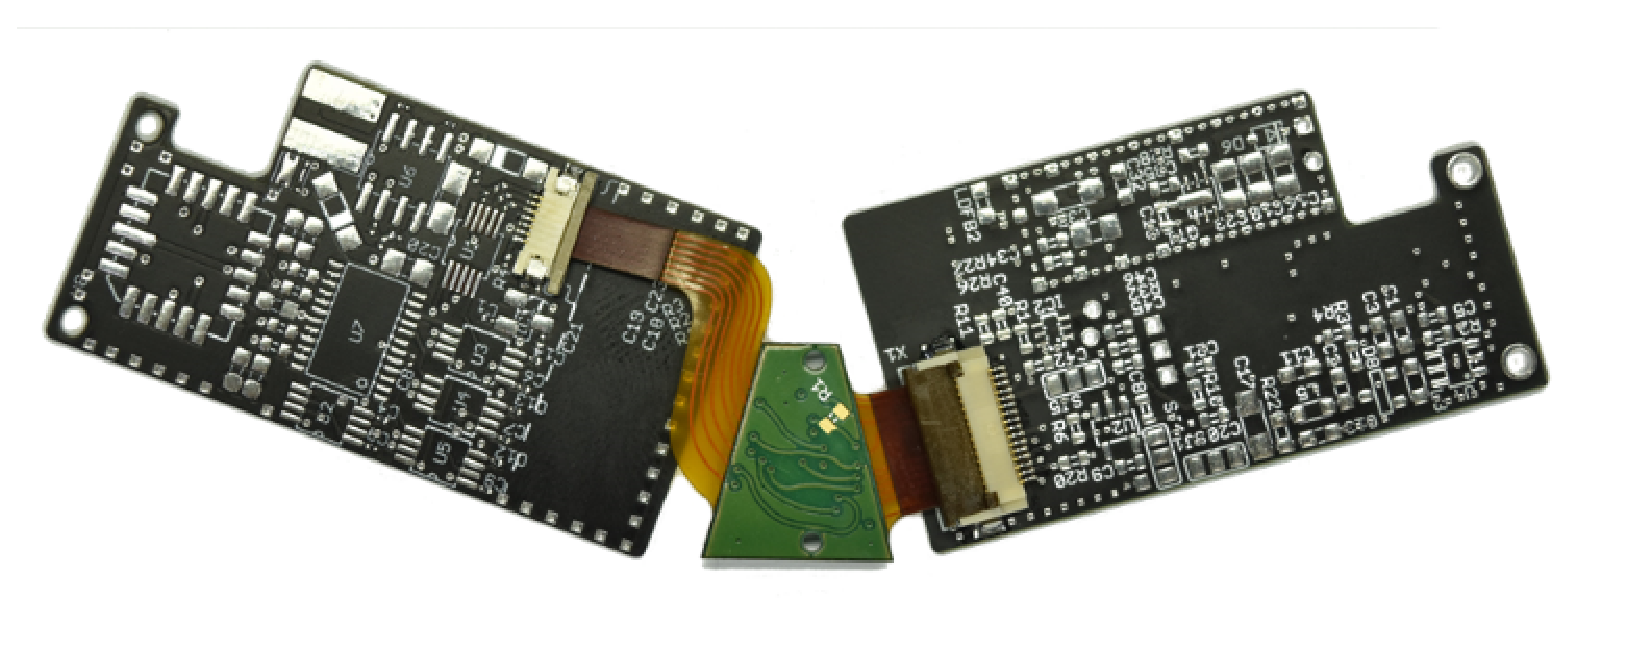
\includegraphics[width=0.75\linewidth]{flex_PCB}
\caption{Connection between MEMS and SiPM board.}
\label{fig:flex_PCB}
\end{figure}

New concept LiDAR with an extremely small size and mass was successfully assembled and is waiting for real tests.
The charateristic of submodule are presented below in the table \ref{tbl:sub_characteristics}

\begin{table}[H]
\label{tbl:rfp_laser}
\begin{center}

\begin{tabular}{|p{0.2\linewidth}|p{0.25\linewidth}|}
\hline
Size: & \textbf{20x28x45 $mm^3$}  \\ \hline
Mass: & \textbf{\textless 200g}  \\ \hline
FOV: & \textbf{\pmb{$30{^\circ}x15{^\circ}$}} \\\hline
Vertical resolution: & \textbf{Flexible, can be any} \\\hline
Distance range: & \textbf{up to 200m} \\  \hline
Power, W: & \textbf{0.4 W} \\  \hline
\end{tabular}
\vspace{-5mm}
\caption{Characteristics of the submodule.}
\label{tbl:sub_characteristics}
\end{center}
\end{table}

\newpage

\begin{figure}[H]
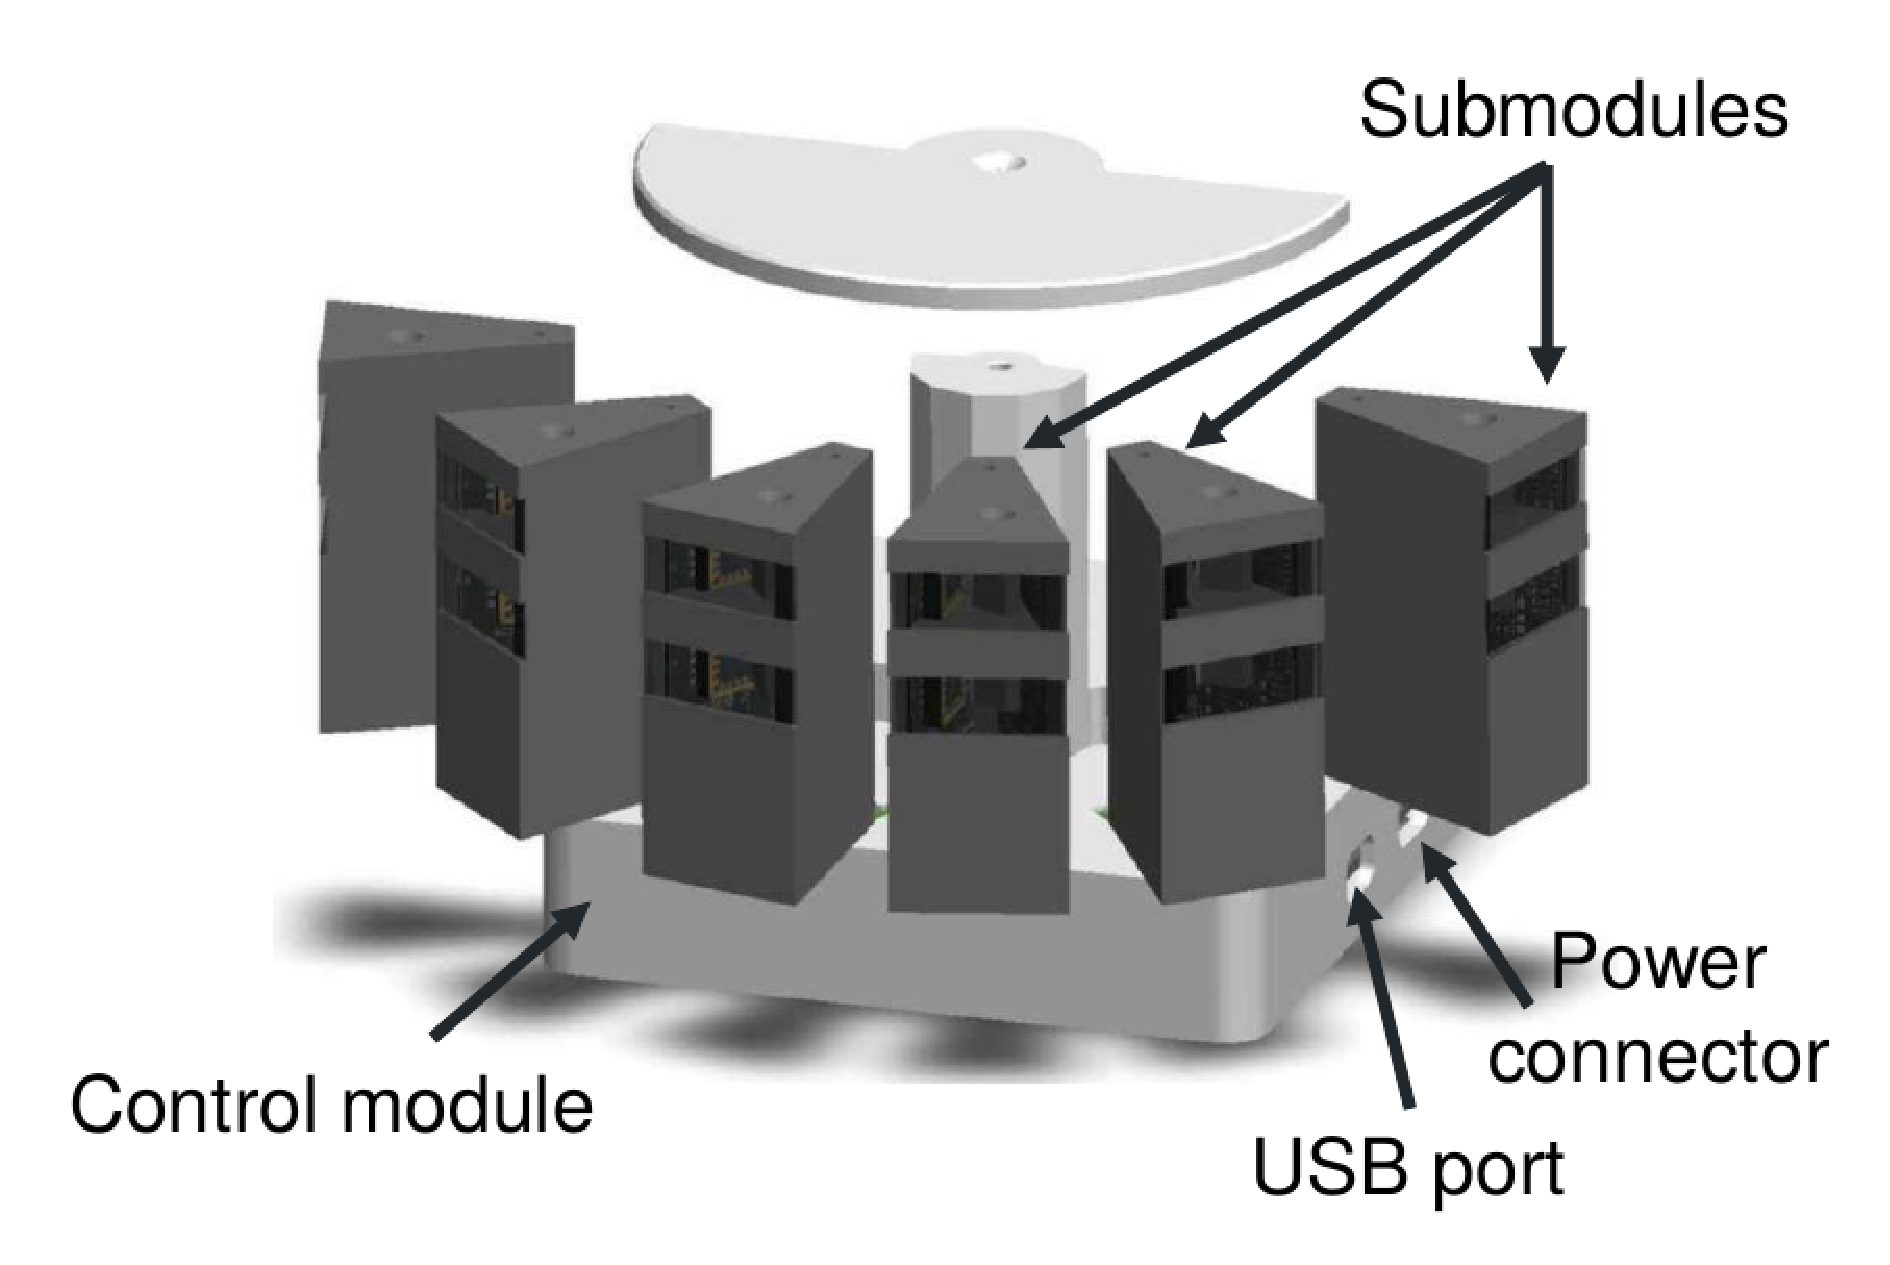
\includegraphics[width=0.7\linewidth]{lidar}
\caption{Modular capability allows to use more than just one submodule.}
\label{fig:lidar}
\end{figure}

Having a modular structure, if necessary, you can increase the field of view by simply adding additional submodules, that makes a lidar incredibly flexible for many applications. Important to note, that control board architecture allow to each submodule works independently and perform various scanning mode with different repetition rate of laser pulse.